\documentclass[12pt,a4paper,oneside]{article}

	\makeatletter
	\newcommand\thefontsize[1]{{}}
	\makeatother
	\usepackage[utf8]{inputenc}
	\usepackage{enumitem}
	\usepackage{varwidth}
	\usepackage{graphicx}
	\usepackage{caption}
	
\usepackage[top=2.5cm, bottom=3cm, left=2.5cm, right=2.5cm]{geometry}
\usepackage[utf8]{inputenc}
\usepackage[titletoc,title]{appendix}
\usepackage[linewidth=1pt]{mdframed}
\usepackage{framed}
\usepackage{listings}
\usepackage{smartdiagram}
\usepackage{smartdiagram}
\usepackage{varwidth}
\usepackage{amsmath}

\usepackage[linesnumbered,ruled,vlined]{algorithm2e}
\usesmartdiagramlibrary{additions}
\lstdefinestyle{customc}{
	belowcaptionskip=1\baselineskip,
	breaklines=true,
	frame=L,
	xleftmargin=\parindent,
	language=C,
	showstringspaces=false,
	basicstyle=\footnotesize\ttfamily,
	keywordstyle=\bfseries\color{green!40!black},
	commentstyle=\itshape\color{purple!40!black},
	identifierstyle=\color{blue},
	stringstyle=\color{orange},
}


\lstset{escapechar=@,style=customc}

\lstset{
	literate=%
	{à}{{\'a}}1
	{í}{{\'i}}1
	{é}{{\'e}}1
	{è}{{\`e}}1
	{ý}{{\'y}}1
	{ú}{{\'u}}1
	{ó}{{\'o}}1
	{ě}{{\v{e}}}1
	{š}{{\v{s}}}1
	{č}{{\v{c}}}1
	{ř}{{\v{r}}}1
	{ž}{{\v{z}}}1
	{ď}{{\v{d}}}1
	{ť}{{\v{t}}}1
	{ň}{{\v{n}}}1
	{ů}{{\r{u}}}1
	{Á}{{\'A}}1
	{Í}{{\'I}}1
	{É}{{\'E}}1
	{Ý}{{\'Y}}1
	{Ú}{{\'U}}1
	{Ó}{{\'O}}1
	{Ě}{{\v{E}}}1
	{Š}{{\v{S}}}1
	{Č}{{\v{C}}}1
	{Ř}{{\v{R}}}1
	{Ž}{{\v{Z}}}1
	{Ď}{{\v{D}}}1
	{Ť}{{\v{T}}}1
	{Ň}{{\v{N}}}1
	{Ů}{{\r{U}}}1
}
\usepackage{booktabs,makecell,tabularx}

\renewcommand\theadfont{\small}
\newcolumntype{L}{>{\raggedright\arraybackslash}X}
\usepackage{siunitx}
\usepackage{adjustbox}
\usepackage{array,booktabs}

\usepackage{graphicx}
\usepackage{epstopdf}

%\newcolumntype{C}[1]{>{\centering\arraybackslash}p{#1}}
\usepackage{algorithm}% http://ctan.org/pkg/algorithms
\usepackage{algpseudocode}% http://ctan.org/pkg/algorithmicx
\usepackage{amsmath}
\begin{document}
	
		\def\reportnumber{}
		\def\reporttitle{Recherche d'information}
		%----------------------------------------------------------------------------------------
%	TITLE PAGE
%----------------------------------------------------------------------------------------

\begin{titlepage} % Suppresses displaying the page number on the title page and the subsequent page counts as page 1
	\newcommand{\HRule}{\rule{\linewidth}{0.5mm}} % Defines a new command for horizontal lines, change thickness here
	
	\center % Centre everything on the page
	
	%------------------------------------------------
	%	Headings
	%------------------------------------------------
	
	\baselineskip=2\baselineskip 
	\textsc{\LARGE Université des Sciences et de la Technologie Houari Boumediene}%\\[1cm] % Main heading such as the name of your university/college

	%------------------------------------------------
	%	Logo
	%------------------------------------------------
	
	%\vfill\vfill
	\vfill
	
\includegraphics[width=0.3\textwidth]{USTHB_Logo.png}\\[1cm] % Include a department/university logo - this will require the graphicx package
	 
	%----------------------------------------------------------------------------------------
	
	\textsc{\Large Recherche d'information }\\[0.5cm] % Major heading such as course name
	%\textsc{\large Minor Heading}\\[0.5cm] % Minor heading such as course title
	
	%------------------------------------------------
	%	Title
	%------------------------------------------------
	
	\HRule\\[0.4cm]
	\baselineskip=1.2\baselineskip 
	{\huge\bfseries Rapport du mini projet\text  \reportnumber \\ \reporttitle}\\[0.4cm] % Title of your document
	
	\HRule\\[1.5cm]
	
	%------------------------------------------------
	%	Author(s)
	%------------------------------------------------
	
	\begin{minipage}{0.4\textwidth}
		\begin{flushleft}
			\large
			\textit{Rédaction:}\\
			MOULAI \textsc{Hassina Safaa}\\ % Your name
			Matricule : 201400007564\\ 
			
			HOUACINE \textsc{Naila Aziza}\\ % Your name
			Matricule : 201400007594\\ 
			
			M2 SII Groupe:3\\
			
		\end{flushleft}
	\end{minipage}
	~
	\begin{minipage}{0.4\textwidth}
		\begin{flushright}
			\large
			\textit{Professeur}\\
			Mr. KECHID Samir  % Supervisor's name
		\end{flushright}
	\end{minipage}
	
	%------------------------------------------------
	%	Date
	%------------------------------------------------
	
	\vfill\vfill\vfill % Position the date 3/4 down the remaining page
	
	{\large\today} % Date, change the \today to a set date if you want to be precise
	
	
	\vfill % Push the date up 1/4 of the remaining page
	
\end{titlepage}
		
		
		\sffamily
		
		\setcounter{tocdepth}{3}
		\tableofcontents
		\listoffigures
		\newpage

\section*{Introduction}

La recherche d'information est apparue comme domaine d'intérêt de nombreux informaticien et mathématicien peu après la création des premiers ordinateur,

Mais c'est surtout avec l'explosion de ressource d'information et de contenus textuelle, images, vidéo,...  disponibles sur le web principalement,que la recherche d'information est devenu primordiale pour tous système de grande échelle, tel que les données ont toujours besoins d'être filtré ou trié par ordre de pertinence selon le besoin,

Aussi afin de restreindra à l'essentiel les données dont nous avons besoin ou de retrouver une information dans une grande masse de données, tout cela afin d'obtenir de meilleurs résultat et d'optimiser les étapes suivante de certain système.\\

La recherche d'information est très largement utilisé aussi bien dans le e-learning, les ontologies, construction de dataset, traitement automatique du langage (TALN) ... etc. mais pas que cette technologie est aussi très présente et très demandé dans les domaines tel que le droit, les langues, ...etc.[1]


\subsection*{Objectifs}
Ce Projet à pour objectif de nous familiariser avec les procédures de base en recherche d'information (RI) et des différentes étapes et méthode qu'elle couvre, tel que l'indexation des documents, la pondération des termes et l'appariement requête-document principalement en utilisant: le modèle Booléen, le modèle Vectoriel et le modèle Probabiliste.

\newpage

\section{Collecte de document}
Comme source de données nous avons choisi le \textbf{brown corpus} de \textbf{nltk} disponible en open source, et cela pour ca richesse et sa diversité car la recherche d'information est appliquée sur de larges collections de documents de diverse provenance, aussi cette bibliothèque offre déjà le liste des \textbf{stopwords} complète. 



\subsection{Pseudo-code}
L'auto-création de notre répertoire pour la collection de documents à étudier.



\begin{algorithm}[H]
	\DontPrintSemicolon
	\KwIn{localpath : chemin vers le dossier à créer,\\
		\hspace{1.3cm}
		name : nom du dossier à créer}
	\KwOut{Le répertoire est crée}

	dir\_name $\gets$ Concatenner(localpath+"/"+name)
	    
	    \textbf{try}:\\
	    \hspace*{0.5cm}
	    s.mkdir(dirName)
	    
	    \textbf{except FileExistsError:}\\
	    \hspace*{0.5cm}
	    print("Directory ", dirName, " already exists")

%	\Return{$L= \bigcup\limits_{k} L_{k}$}\;
	\caption{{\sc Création du répertoire}}
	\label{algo:duplicate2}
\end{algorithm}

L'automatisation du remplissage de nos documents à partir du contenu des documents du brown corpus.


\begin{algorithm}[H]
	\DontPrintSemicolon
	\KwIn{directory : chemin vers le dossier ou créer les documents,\\
		\hspace{1.3cm} n : nombre de documents a créer}
	\KwOut{Les documents créer et remplis}
	
	liste $\gets$ nltk.corpus.gutenberg.fileids()
	
	\For{$element \in liste$}{
		path\_element $\gets$ Concatenner(directory+"/"+element)\\
		f $\gets$ Ouvrire\_en\_ecriture(path\_element)\\
		Ecrire(f,Convertir\_en\_text(nltk.corpus.gutenberg.words(element)))[:60])\\
		Fermer(f)
	}
	
	%\Return{$L= \bigcup\limits_{k} L_{k}$}\;
	\caption{{\sc creation de N docuements}}
	\label{algo:duplicate2}
\end{algorithm}



\newpage

\section{Indexation des documents}
un index inversé est une correspondance entre du contenu, comme des mots ou des nombres, et sa position dans un ensemble de données comme un enregistrement en base de données, un document ou un ensemble de documents ; sur le même principe qu'un index terminologique. Le but de l'index inversé est de permettre une recherche plein texte plus rapide, contre un temps d'insertion de nouvelles données augmenté. [wiki]

\subsection{Structure de données}
%//explication de la structure 
On a utilisé pour indexer nos termes appartenant à un document , on opté pour un dictionnaire de dictionnaire comme suit:
\begin{lstlisting}

	Fichier-Inverse : {
		 terme1 : {doc1 : freq , doc2 : freq , ...},
		 terme2 : {doc1 : freq , doc2 : freq , ...},
		 ...
		}
\end{lstlisting}

\begin{itemize}
\item Le premier dictionnaire a  pour clé  le \textbf{terme} et comme valeurs un dictionnaire de \textbf{document} : \textbf{fréquence} tel que la fréquence est celle du terme dans le document.
\end{itemize}

\subsubsection*{exemple}
%//juste un exemple FichierInv[terme,doc]$->$frq + mini schéma

\subsection{Pseudo-code}


\begin{algorithm}[H]
                 	\DontPrintSemicolon
                 	\KwIn{listDocs : liste des documents}

                 	\KwOut{FichierInferseFreq}

Fichier\_Inverse $ \gets$ New Dictionary(term,New Dictionary(Doc,Frequency)))
                 	
                 	
                 	
                 	\For{$doc \in listDocs $}{
                 		\For{$terme \in doc $}{
                 			
	  Fichier\_Inverse[$terme$][$doc$]$\gets$Fichier\_Inverse[$terme$][$doc$]+1;
                 		}
                 		
                 		
                 	}
                 	\Return{$InverseFichiers$}\;
                 	\caption{{\sc  }}
                 	\label{algo:duplicate2}
\end{algorithm}


\subsection{Explication de l'algorithme}

La création du fichier inverse se fait comme suit:
\begin{itemize}
\item[$\bullet$] Parcours des documents un par un 
\item[$\bullet$] Pour chaque document on parcours ses termes
\item[$\bullet$] Pour chaque pair de terme document on incrémente la fréquence en accédant à notre dictionnaire avec les deux pair de clés (TERME , DOCUMENT).
\end{itemize}

\subsection{Résultat}
ainsi notre fichier inverse peu etre représenté par une matrice dont les lignes sont les termes et les colonnes les documents, puis chaque cellule $C_ij$ contient la fréquence du terme $t_i$ de la $i^eme$ ligne dans le document $d_j$ de la $j^eme$ colonne.

	\begin{figure}[H]
		\centering
		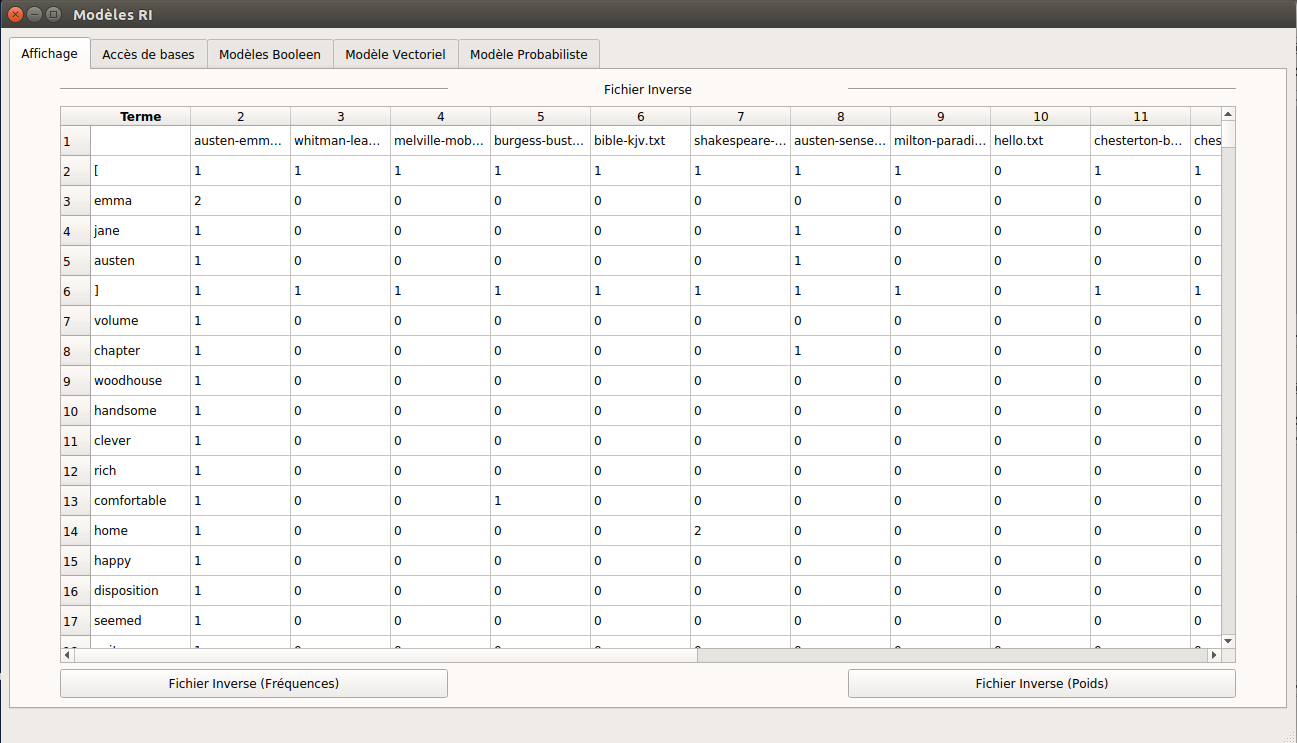
\includegraphics[scale=0.35]{images/fichierI.png}
		\caption{Fichier Inverse de notre collection}
	\end{figure}







\newpage

\section{Pondération des termes}
Il est souvent utile de donner plus d'importance à certain terme lors d'un processus de RI, pour cela plusieurs approche existent.

Parmi les approches les plus répondu pour la pondération des termes d'une collection de document nous retrouvons \textbf{TF*IDF}, dont la formule est la suivante:
\begin{center}
	$poids(t_i,d_j)=((fichierInverse[t_i][d_j])/Max)* \log((N/N_i)+1)$
	
\end{center}
Avec:\\
$t_i$ le $i^eme$ terme.\\
$d_j$ le $j^eme$ document.\\
$Max: $ fréquence maximal du terme dans le document.\\
$N_i: $ nombre de Documents ou apparait le terme $t_i$.\\
$N: $ le nombre de document de la collection.\\

\subsection{Structure de données}
La structure de notre \textbf{fichier inverse pondéré} est identique à celui du fichier inverse des fréquence à la différence que chaque cellule contient un \textbf{poids} et non pas une fréquence.
\begin{lstlisting}

Fichier-Inverse-pondéré : {
terme1 : {doc1 : poids , doc2 : poids , ...},
terme2 : {doc1 : poids , doc2 : poids , ...},
...
}
\end{lstlisting}


\subsection{Pseudo-code}

\begin{algorithm}[H]
	\DontPrintSemicolon
	\KwIn{listDocs : liste des documents}
	
	\KwOut{fichierInbersePoids}
	
	Fichier\_Inverse\_Poids $ \gets$ New Dictionary(term,New Dictionary(Doc,Poids)))
	
	
	
	\For{$doc \in listDocs $}{
		\For{$terme \in doc $}{
			$poids \gets TFIDF()$\\ 
			Fichier\_Inverse\_Poids[$terme$][$doc$]$\gets poids$;
		}
	}
	\Return{$InverseFichiersPoids$}\;
	\caption{{\sc  }}
	\label{algo:duplicate2}
\end{algorithm}

\newpage

\subsection{Explication de l'algorithme}
\begin{itemize}
	\item[$\bullet$] pour chaque terme de la collection.
	\item[$\bullet$] pour chaque document de la collection.
	\item[$\bullet$] Calculer le fonction \textbf{TF*IDF} et l'affecter au (Terme,Document) correspondant.
	\item[$\bullet$] retourner le fichier Inverse des Poids.
\end{itemize} 

\subsection{Résultat}
Notre fichier inverse des poids est aussi affichable sous forme de matrice [terme,Document] $\Rightarrow$ Poids, comme dans la figure qui suit:

	\begin{figure}[H]
		\centering
		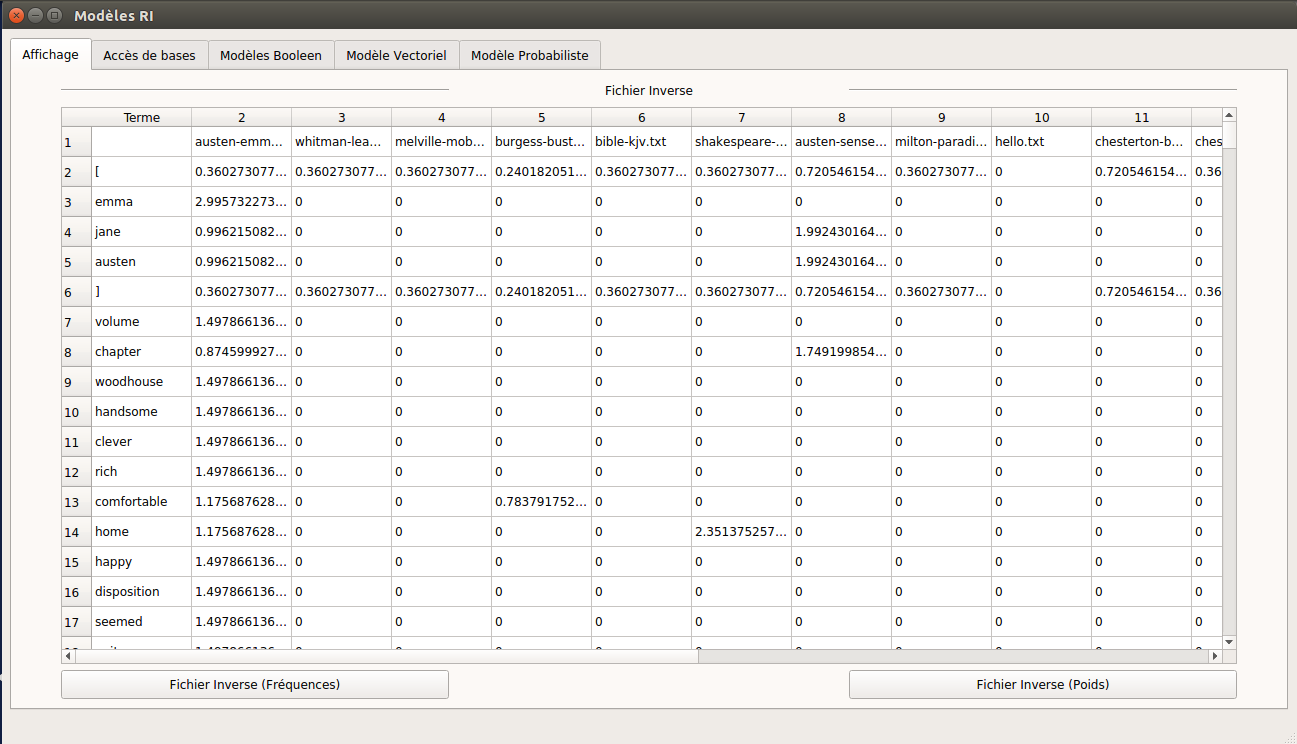
\includegraphics[scale=0.35]{images/fichierP.png}
		\caption{Fichier Inverse de notre collection}
	\end{figure}




\newpage

\section{Fonctions d'accès}
Il est nécessaire de définir des fonctions d'accès pour n'importe quelle structure de données que nous définissons, c'est pourquoi les deux fonctions qui suivent nous permettent de manipuler les informations de nos fichiers inverse de fréquence et de poids.

\subsection{Recherche les termes(fréquence/poids) d'un Document donné}
Pour un document $d$ saisi pas l'utilisateur on retourne la liste de ses termes avec leurs fréquences et leurs poids.

\subsubsection*{Pseudo-code}


\begin{algorithm}[H]
	\DontPrintSemicolon
	\KwIn{document,fichier\_Inverse}
	
	\KwOut{listTermes}

	\For{$terme \in Fichier\_Inverse $}{
		\For{$doc \in $Fichier\_Inverse[$terme$]}{
  
			listTermes[$terme$] $\gets $Fichier\_Inverse[$terme$][$doc$]\\

		}
	}

	\Return{$listTermes$}\;
	\caption{{\sc  }}
	\label{algo:duplicate2}
\end{algorithm}


\subsubsection*{Explication de l'algorithme}
la fonction prend on paramètre le document dont nous voulons récupérer les termes, puis procède comme suit:
\begin{itemize}
	\item[$\bullet$] pour chaque terme du fichier inverse.
	\item[$\bullet$] si le document contient ce terme on récupère la fréquence de ce terme.
	\item[$\bullet$] on retourne la liste de (terme,freq) du document en entrée.
\end{itemize}
\subsubsection*{Résultat}
Après que l'utilisateur ne saisisse le nom du document donc il souhaite connaitre les terme/fréquence/poids, il valide en cliquant sur \textbf{"OK"}, les informations recherchées lui sont affichées comme suit:

	\begin{figure}[H]
		\centering
		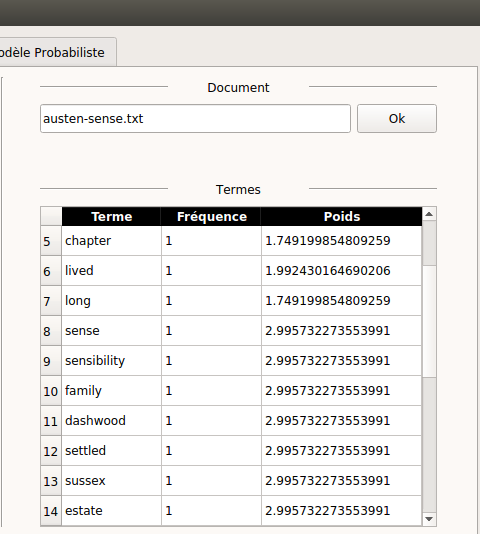
\includegraphics[scale=0.48]{images/f1.png}
		\caption{fonction d'accès à travers un document}
	\end{figure}



\subsection{Recherche les documents(fréquence/poids) contenant un terme donné}
Pour terme donné on retourne la liste des documents dans les quels il apparait avec sa fréquences et son poids pour chaque documents.

\subsubsection*{Pseudo-code}
\begin{algorithm}[H]
	\DontPrintSemicolon
	\KwIn{$t_i$,fichier\_Inverse}
	
	\KwOut{listDocs}
	
	\For{$terme \in Fichier\_Inverse $}{
		\If{$terme == t_i$}{
			\For{$doc \in $Fichier\_Inverse[$terme$]}{
				
				listDocs[$doc$] $\gets 	$Fichier\_Inverse[$terme$][$doc$]\\		
			}
		}
	}
		        
	\Return{$listDocs$}\;
	\caption{{\sc  }}
	\label{algo:duplicate2}
\end{algorithm}
\subsubsection*{Explication de l'algorithme}
la fonction prend on paramètre le terme recharché $t_i$ dont nous voulons récupérer les documents ou il apparait, pour cela nous procédons comme suit:
\begin{itemize}
	\item[$\bullet$] pour chaque terme du fichier inverse.
	\item[$\bullet$] s'il s'agit du terme recherché.
	\item[$\bullet$] pour chaque document comportant ce terme ajouter le document/fréquence de ce terme dans le document en cours de traitement	\item[$\bullet$] on retourne la liste de (doc,freq) du document en entrée.
\end{itemize}

\subsubsection*{Résultat}
Un champs de saisi est mis à disposition de l'utilisateur pour y taper le terme dont il veut connaitre les documents oui il apparait et avec quelle fréquence et poids, puis il n'a plus qu'a valider sa recherche via le bouton \textbf{"OK"}, les informations recherchées lui sont affichées comme suit:

\begin{figure}[H]
	\centering
	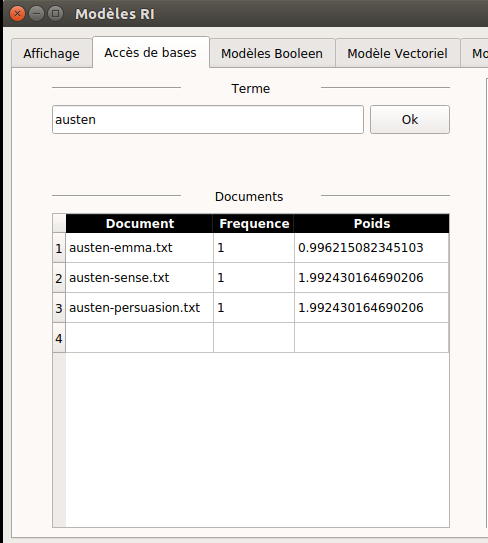
\includegraphics[scale=0.48]{images/f2.png}
	\caption{Fonction d'accès à travers un terme}
\end{figure}





\newpage

\section{Appariement Requête-Document}
Il s'agit de calculer à quelle degrés une requête correspond ou concorde avec le contenu d'un document, pour cela nous allons utiliser comme mesure la \textbf{similitude}, celle si peut être calculé selon diverses modèle telle que: \textbf{le modèle boolean, le modèle vectoriel, le modèle probabiliste avec ses différentes variantes, ...}\\

Chacun des modèles cités ci-dessus possède des avantages et inconvénients, c'est pour cela que nous allons les implémenter et tester sur un même ensemble de document et comparer les résultats obtenus.

\subsection{Modèle Booléen}
Le modèle booléen traite une requête comme une expression logique. tel que pour un document doc1 et un terme t1,nous pouvons évaluer la similitude comme étant vraie (Similaire) si le terme t1 existe dans le document doc1 et comme fausse (non similaire) dans le cas contraire.

\subsubsection*{Requête}
%forme de la requête + exemple
Dans ce modèle nous définissons trois opérateurs AND, OR et NOT pour relier les termes de la requête.\\
exemple : requête = "t1 AND (t2 OR t3)"\\
Ainsi cette requête peut etre décomposé comme suit : \\
requête1 = t1\\
requête2 = t2\\
requête3 = t3\\

Avec : \\
Appariement(requête, doc) = Appariement(requête1, doc) AND ( Appariement(requête2, doc) OR Appariement(requête3, doc))\\

ainsi cela revient a évaluer une l'expression booleen composé de "True" et "False" ainsi que des opérateur logique de bases cités précédemment.

\subsubsection*{Fonction d'appariement : Pseudo-code} 

\begin{algorithm}[H]
	\DontPrintSemicolon
	\KwIn{listDocs : liste des documents,\\
	\hspace{1.3cm}fichierInverse : le fichier inverse de notre ensemble de documents,\\
	\hspace{1.3cm}requete}
	\KwOut{listDocsPertinents : la liste des documents pertinents\\
	\hspace{1.4cm} (c'est-a-dire dont la similitude == 1)}
	
	
	
	\For{$doc \in listDocs $}{
		\For{$terme \in requete $}{
			\If{$terme \notin [AND , OR , NOT]$}{
				\If{$terme \in fichierInverse[doc]$}{
					$resultat \gets 1$
				}
				\Else{
					$resultat \gets 0$
				}
			}
			\Else{
				$resultat \gets terme$
			}
			
		}
		
		$resultat$ = ConvertirEnChaineDeCara($resultat$)\\
		\If{Evaluation($resultat$) == True}{
			Ineserer($doc , listDocsPertinents$)
		}
	}
	\Return{$listDocsPertinents$}\;
	\caption{{\sc Modèle Boolean}}
	\label{algo:duplicate2}
\end{algorithm}



\subsubsection*{Explication de l'algorithme}
notre algorithme effectue alors la séquence d'instruction suivante:
\begin{itemize}
	\item[$\bullet$] pour chaque document de la collection.
	\item[$\bullet$] pour chaque terme de la requete différent des opérateurs (et, ou, not).
	\item[$\bullet$] rechercher le terme dans le fichier inverse pour le document en cours de traitement.
	\item[$\bullet$] s'il existe remplacer le terme par la valeur booléenne \textit{"True"} par \textit{"False"} sinon.
	\item[$\bullet$] Évaluer la nouvelle requête obtenu (composée de booléen et d'opérateur logique)
	\item[$\bullet$] retourner la liste de document dont l'évaluation a donnée \textit{"True"}
\end{itemize}

\subsubsection*{Résultat}
Pour le requete :
\begin{center}
	\textbf{(jane and austen) and not volume}
\end{center} 

nous aurons comme résultat tous les documents de notre collection qui contiennent les mot : \textbf{jane} et \textbf{austen} mais qui ne contiennent pas le mot \textbf{volume}.\\

l'exécution de notre modèle booléen nous retourne 2 documents qui sont : \textbf{austen-sense.txt} et \textbf{austen-persuasion.txt}\\

comme le montre la figure suivante:
	\begin{figure}[H]
		\centering
		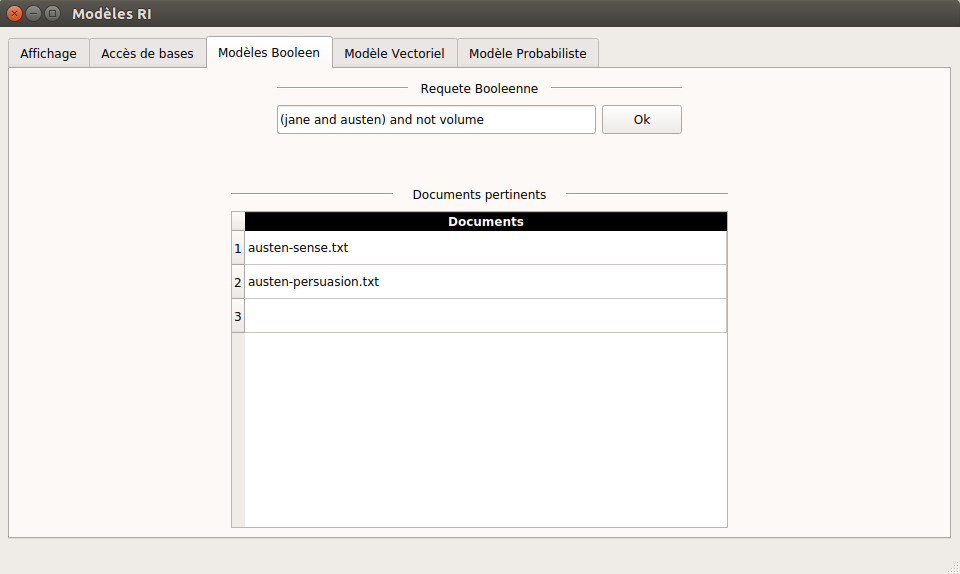
\includegraphics[scale=0.4]{images/modeleB.png}
		\caption{Résultat du modèle booléen.}
	\end{figure}
	
Nous pouvons vérifié qu'effectivement ce sont les deux seules document vérifiant la requête de notre collection.
	\begin{figure}[H]
		\centering
		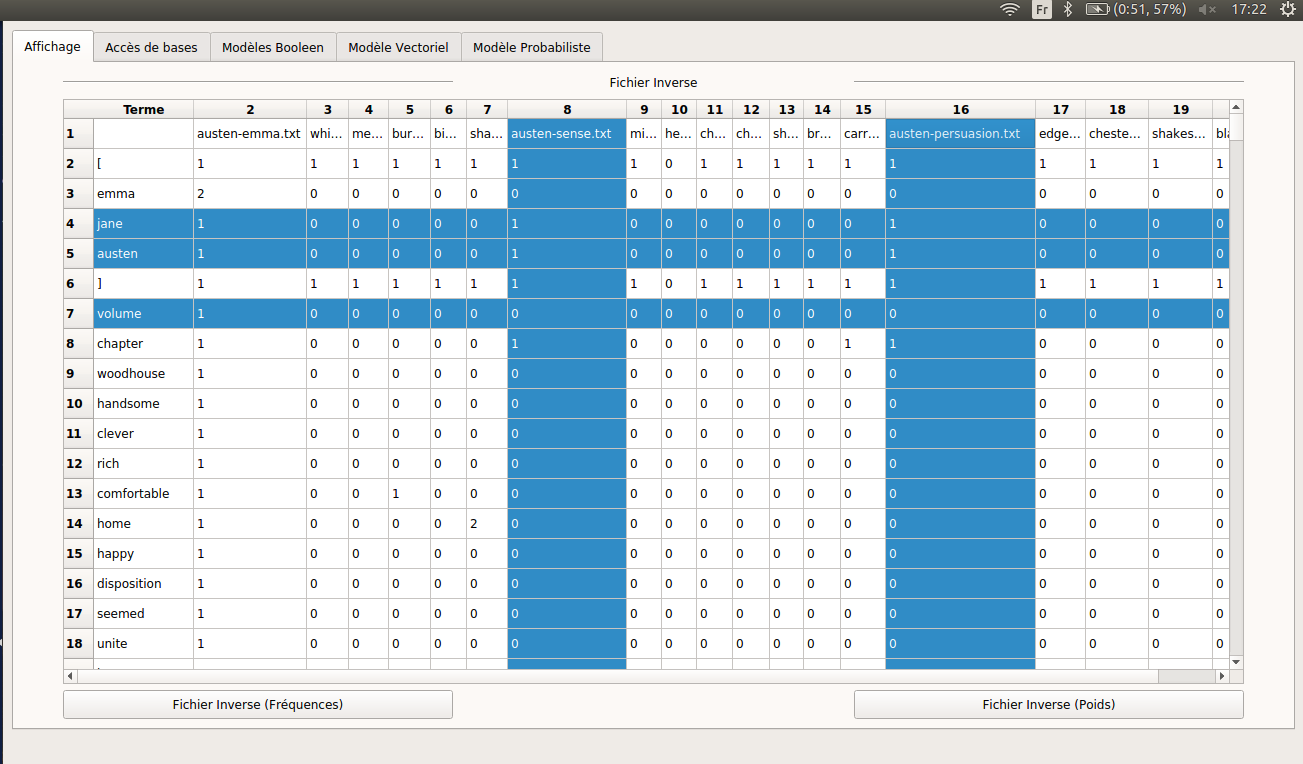
\includegraphics[scale=0.3]{images/modeleB2.png}
		\caption{Vérification du résultat du modèle booléen.}
	\end{figure}


\newpage
\subsection{Modèle Vectoriel}
Dans le modèle vectoriel les documents sont modélisant à travers un vecteur contenant tous les termes de la collection de tel façon à ce que si le  terme apparaît dans le document alors la case du terme en question sera mise  à 1 et 0 sinon si on modélise avec un système sans poids .


\begin{equation}
\begin{split}
T=& <t_{1},t_{t2}...,t_{n}>
\end{split}           
\end{equation}
soit un document j les termes qui apparaissent dans le document seront représentées par leur poids
\begin{equation}
\begin{split}
Document : dj &= (w_{1j},w{2j},....,w_{nj})
\end{split}   
\end{equation}

$w_{ij}$:poids du terme $t_{i}$ dans le document $d_{j}$ à tf*idf


\subsubsection*{Requête}
La requête est également représenté par un vecteur de l'ensemble des termes de la collection pondéré de la manière suivante:

\begin{equation}
\begin{split}
Query=&(w_{1q},w_{2q},...,w_{nq})
\end{split}
\end{equation}
$w_{iq}$:poids du terme $t_{i}$ dans la requête $q$ .


\subsubsection*{Fonction de similitude}
Pour le modèle vectoriel il existe plusieurs fonction de similitude avant de les citer on doit définir la mesure par quelle se fait la classification des documents selon leurs degré de pertinence pour une requête .

on dira qu'un document est $d_{1}$ est d’autant plus pertinent à une requête que le  vecteur 
associé est similaire à celui de la requête .

\subsubsection*{\hspace{1cm}1-	Produit Interne} 
%//2 ligne explication + formule + Pseudo code avec commentaire 
le produit interne permet de quantifier
le degré de similarité entre deux vecteurs , ainsi plus le produit est grand plus le degré de similarité entre les deux est grande .
\begin{equation*}
\begin{split}
\sum_{i=1}^{n} & q*d\\
Sim(q,d_i) =& \vec{q} . \vec{d_i} = \sum_{j=1}^{n} q_j * d_{i,j}
\end{split}
\end{equation*}

\subsubsection*{\hspace{1cm}2-	Coefficient de Dice} 
\begin{equation*}
Sim(Q,T_i) = \frac{2*|T_i \bigcap Q|}{|T_i \bigcup Q|} = \frac{|T_i \bigcap Q|}{|T_i|+|Q|}
\end{equation*}

\[
Sim(q,d_i) = \frac{2*\sum_{j=1}^{n} q_{j} * d_{i,j}}
{\sum_{j=1}^{n} q_{j}^2 + \sum_{j=1}^{n} d_{i,j}^2 }
\]

\subsubsection*{\hspace{1cm}3-	Cosinus} 
\begin{equation*}
\begin{gathered}
\vec{q}.\vec{d} = \parallel \vec{q}\parallel * \parallel \vec{d} \parallel  * cos(\overrightarrow{q,d}) \\\\
cos(\overrightarrow{q,d}) = \frac{\sum_{i=1}^{n} q_{1,i} * d_{2,i} }
{\sqrt{\sum_{i=1}^{n} q_{1,i}^2} * \sqrt{\sum_{i=1}^{n} d_{2,i}^2} }
\end{gathered}
\end{equation*}
\subsubsection*{\hspace{1cm}4-	Jaccard} 
%//2 ligne explication + formule + Pseudo code avec commentaire 
\[
Sim(Q,T_i) = \frac{|T_i \bigcap Q|}{|T_i \bigcup Q|} = \frac{|T_i \bigcap Q|}{|T_i|+|Q|-|T_i \bigcap Q|}
\]

\[
Sim(q,d_i) = \frac{\sum_{j=1}^{n} q_{j} * d_{i,j}}
{\sum_{j=1}^{n} q_{j}^2 + \sum_{j=1}^{n} d_{i,j}^2 - \sum_{j=1}^{n} q_{j} * d_{i,j}}
\]


$q_{i}$ est le poids du terme $t_{i}$ dans la requête .

$d_{i}$ est le poids du terme $t_{i} $dans le document .
\subsubsection*{Fonction d'appariement : Pseudo-code} 
\begin{algorithm}[H]
	\DontPrintSemicolon
	\KwIn{
		fichierInverse : le fichier inverse de notre ensemble de documents,\\
		\hspace{1.3cm}requete}
	\KwOut{listDocsPertinents : la liste des documents triés par degré de pertinence
	}
	
	
	
	
	\For{$doc \in listDocs $}{
		
		
		sim $\gets$ FonctionAppariment(doc,requete)
		
		\If{(sim != 0)}
		{
			listDocsPertinents[doc] $\gets$ sim
		}
		
	}
	
	
	
	
	
	listDocsPertinents $\gets$ TrierOrdreDecroissant(listDocsPertinents
	)
	
	
	\Return{$listDocsPertinents$}
	\caption{{\sc Modèle vectoriel}}
	\label{algo:duplicate2}
\end{algorithm}


\begin{algorithm}[H]
	\DontPrintSemicolon
	\KwIn{
		Document,\\
		\hspace{1.3cm}requete}
	\KwOut{similarité
	}
	
	
	somme1 $\gets$0
	
	somme2$\gets$ 0
	
	somme3$\gets$0
	
	
	\For{$i \in [0,longueur(doc)] $}{
		
		somme1 $\gets$ somme1 + (requete[i] * doc[i] )
		
		somme2 $\gets$ somme2 + ($requete[i]^2$)
		
		somme3  $\gets$ somme3 + ($document[i]^2$)
		
	}	  
	
	var  $\gets$ somme2 + somme3 - somme1
	
	\If{(var == 0)}
	{
		sim=0}
	\Else{
		
		sim $\gets$  $\frac{somme1}{var}$
		
	}
	
	
	
	
	
	\Return{$sim$}\;
	\caption{{\sc FonctionDappariment:(JACCARD)}}
	\label{algo:duplicate2}
\end{algorithm}
\begin{algorithm}[H]
	\DontPrintSemicolon
	\KwIn{
		Document,\\
		\hspace{1.3cm}requete}
	\KwOut{similarité
	}
	
	
	
	
	
	
	somme1 $\gets$0
	
	somme2$\gets$ 0
	
	somme3$\gets$0
	
	
	\For{$i \in [0,longueur(doc)] $}{
		
		somme1 $\gets$ somme1 + (requete[i] * doc[i] )
		
		somme2 $\gets$ somme2 + ($requete[i]^2$)
		
		somme3  $\gets$ somme3 + ($document[i]^2$)
		
	}	  
	
	var  $\gets$ somme2 + somme3 - somme1
	
	\If{(somme2 ==0 or somme3 ==0)}
	{
		sim=0}
	\Else{
		
		sim $\gets$  $\frac{somme1}{\sqrt{(somme2 * somme3)}}$
		
	}
	
	
	\Return{$sim$}\;
	\caption{{\sc FonctionDappariment:(Cosinus)}}
	\label{algo:duplicate2}
\end{algorithm}

\begin{algorithm}[H]
	\DontPrintSemicolon
	\KwIn{
		Document,\\
		\hspace{1.3cm}requete}
	\KwOut{similarité
	}
	
	somme1 $\gets$0
	
	somme2$\gets$ 0
	
	somme3$\gets$0
	
	
	\For{$i \in [0,longueur(doc)] $}{
		
		somme1 $\gets$ somme1 + (requete[i] * doc[i] )
		
		somme2 $\gets$ somme2 + ($requete[i]^2$)
		
		somme3  $\gets$ somme3 + ($document[i]^2$)
		
	}	  
	
	var  $\gets$ somme2 + somme3 - somme1
	
	\If{(somme2 ==0 or somme3 ==0)}
	{
		sim=0}
	\Else{
		
		sim $\gets$  $\frac{2*somme1}{(somme2 +somme3)}$
		
	}
	
	
	
	\Return{$sim$}\;
	\caption{{\sc FonctionDappariment:(Dice)}}
	\label{algo:duplicate2}
\end{algorithm}


\begin{algorithm}[H]
	\DontPrintSemicolon
	\KwIn{
		Document,\\
		\hspace{1.3cm}requete}
	\KwOut{similarité
	}
	
	sim $\gets$ 0
	
	
	\For{$i \in [0,longueur(doc)] $}{
		sim $\gets$ sim + (requete[i] * document[i] )
		
		
	}	  
	
	\Return{$sim$}\;
	\caption{{\sc FonctionDappariment:(Produit Interne)}}
	\label{algo:duplicate2}
\end{algorithm}


\subsubsection*{Explication de l'algorithme}
l'algorithme basé de le modèle vectoriel fonctionne comme suit: 

\begin{itemize}
	\item  Pour chaque document de notre collection on calcule la similarité entre notre document et la requête
	\item On choisi une fonction de similarité parmi celle implémenté (jaccard, dice, produit interne ,cosinus)
	\item si la similarité est non nulle alors on l'ajoute à une liste de tel sorte que l'indice est celui du document 
	\item on trie la liste des documents pertinents par ordre décroissant
	\item le premier élément de la liste étant le document le plus pertinent ayant la plus grande similarité 
\end{itemize}

\subsubsection*{Résultat}
on a exécuté \textbf{la requête q = ("blue")}.

voici les résultats avec les différentes fonctions d'appariement
\begin{figure}[H]
	\centering
	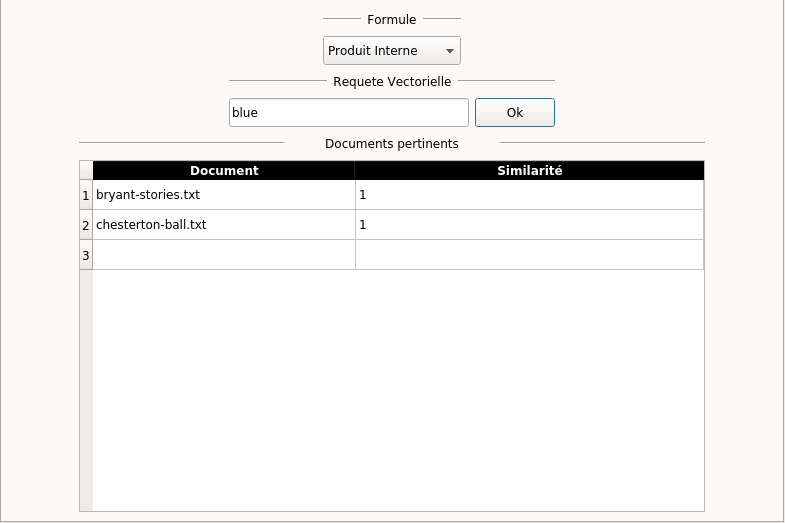
\includegraphics[scale=0.4]{images/produitinterne.png}
	\caption{Résultat du modèle vectoriel avec Produit interne comme Fonction d'appariement.}
\end{figure}
\begin{figure}[H]
	\centering
	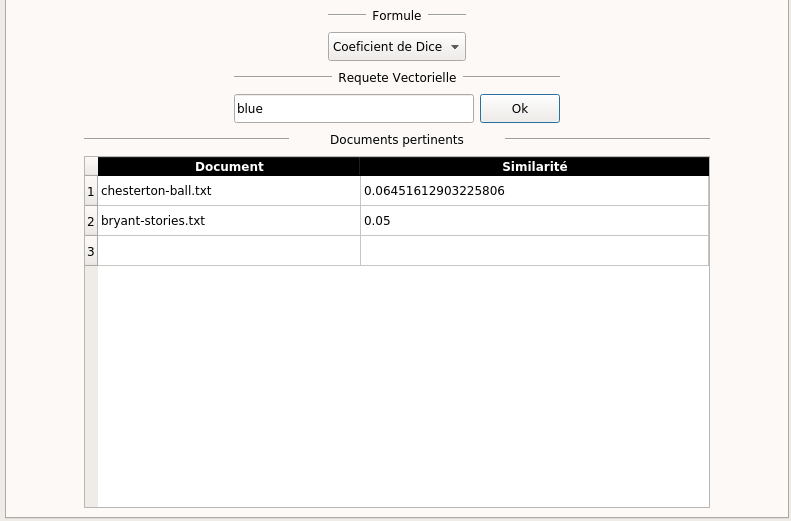
\includegraphics[scale=0.4]{images/dice.png}
	\caption{Résultat du modèle vectoriel avec Dice comme Fonction d'appariement.}
\end{figure}

\begin{figure}[H]
	\centering
	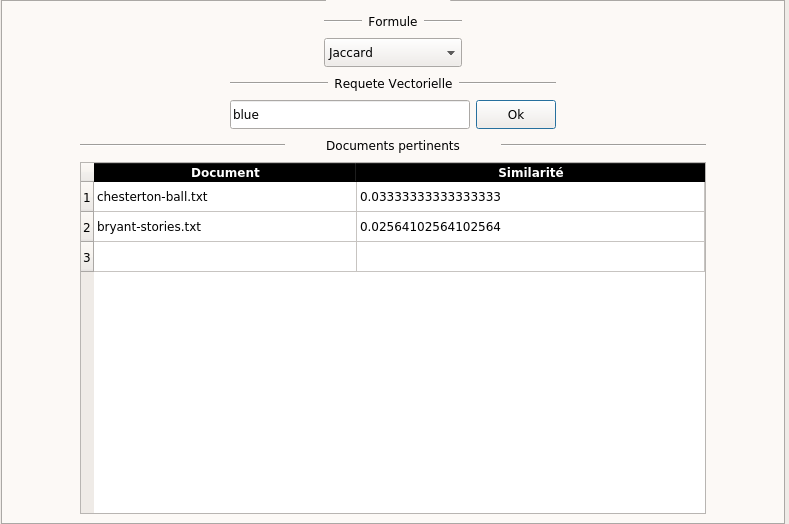
\includegraphics[scale=0.4]{images/jaccard.png}
	\caption{Résultat du modèle vectoriel avec Jaccard comme Fonction d'appariement.}
\end{figure}
\begin{figure}[H]
	\centering
	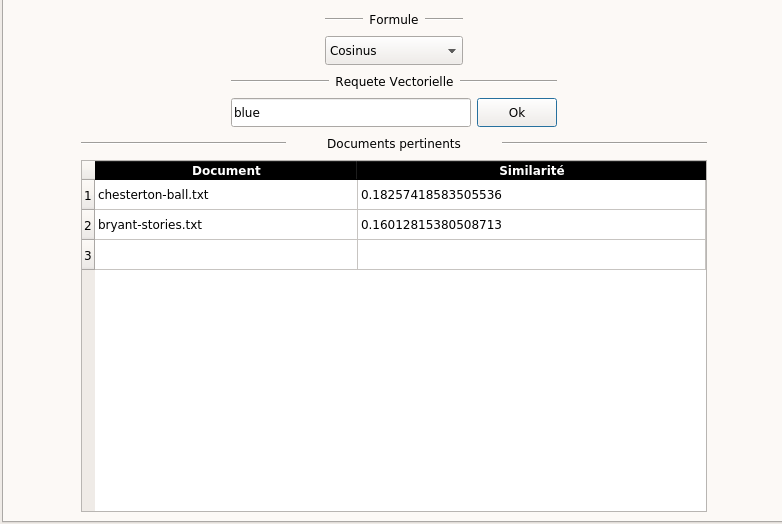
\includegraphics[scale=0.4]{images/cosinus.png}
	\caption{Résultat du modèle vectoriel avec COSINUS comme Fonction d'appariement.}
\end{figure}




\subsubsection*{Comparaison}
On remarque que avec le produit interne on a eu une similarité identique entre les deux documents contrairement aux trois autres fonctions jaccard ,dice , cosinus qui ont donné des résultats identiques avec le même tri des documents .

On peut conclure que les fonctions  jaccard ,cosinus , dice sont plus précises pour le calcul de similarité entre les  documents comparé au produit interne ceci se traduit par la complexité de leurs calcul .



\newpage

\subsection{Modèle Probabiliste avec échantillon}

Le modèle probabiliste quant à lui, requière un échantillon d'apprentissage. Dans notre cas,
cet échantillon sera les documents jugés pertinents par l'utilisateur lui même.\\

C'est à dire que notre modèle probabiliste répondra en premier lieu à la requête de l'utilisateur
avec le modèle vectoriel cité juste au dessus, puis à partir de cet échantillon l'utilisateur choisira parmi les documents
retournés par le modèle vectoriel ceux qu'il juge pertinents $\Rightarrow$ échantillon d'apprentissage .\\

Puis nous procédons à une deuxième recherche avec cette même
requête en appliquant le modèle probabiliste dont la formule pondéré qui est comme suit:\\

\begin{center}
	Sim($d_{j},Q$)= $\sum_{i=1}^{n} P_{ij} * P_{iq} \log \dfrac{(r_{i}+0.5)/(R-r_{i}+0.5)}{(n_{i}-r_{i}+0.5)/(N-n_{i}-R+r_{i}+0.5)}$
\end{center}

avec:\\
$d_{j} :$ le document j.\\
$Q :$ la requête.\\
$n :$ le nombre de terme dans la requête Q.\\
$r_{i} :$ le nombre de documents pertinents contenant le terme $t_{i}$.\\
$R :$ le nombre de documents pertinents.\\
$n_{i} :$le nombre de documents contenant le terme $t_{i}$.\\
$N :$ le nombre de document de notre collection.\\
$P_{ij} :$ le poids du terme $t_{i}$ dans le document j.
$P_[iq] :$ le poids du terme $t_{i}$ dans la requête Q.

\subsubsection*{Requête}
La requête à la même forme que celle décrite précédemment pour le modèle Vectoriel.

\subsubsection*{Fonction d'appariement : Pseudo-code} 
\begin{algorithm}[H]
	\DontPrintSemicolon
	\KwIn{listDocs : liste des documents,\\
		\hspace{1.3cm}fichierInversePoids : le fichier inverse des poids de notre ensemble de documents,\\
		\hspace{1.3cm}listDocPertinents : la liste des documents pertinents\\
		\hspace{1.3cm}requete: requete recherchée}
	\KwOut{listDocsPertinents : la liste des documents pertinents\\ }	
	
	$N \gets$ longeur(listDocs)\\
	$R \gets$ longeur(listDocPertinents)\\
	\For{$doc \in listDocs $}{
		$Sim \gets 0$\\
		\For{$terme \in requete $}{
			$n_i \gets $ NbrDocContenantTi(listDocs,terme)\\
			$r_i \gets $ NbrDocContenantTi(listDocPertinents,terme)\\
			$P_ij \gets fichierIneversePoids[dos][terme]$\\
			$P_iq \gets nbrOccurence(terme,requete)$\\
			
			$Sim \gets $ $Sim + [ P_{ij} * P_{iq} \log \dfrac{(r_{i}+0.5)/(R-r_{i}+0.5)}{(n_{i}-r_{i}+0.5)/(N-n_{i}-R+r_{i}+0.5)}]$
			
		}
		
		\If{$Sim > 0$}{
			Ineserer($doc , listDocsPertinents$)
		}
	}
	\Return{$listDocsPertinents$}\;
	\caption{{\sc Modèle Probabiliste}}
	\label{algo:duplicate2}
\end{algorithm}
    
\subsubsection*{Explication de l'algorithme}
notre algorithme effectue alors la séquence d'instruction suivante:
\begin{itemize}
	\item[$\bullet$] pour chaque document de la collection.
	\item[$\bullet$] pour chaque terme de la requête.
	\item[$\bullet$] Calculer le nombre de document contenant le terme courant de la requête.
	\item[$\bullet$] Calculer le nombre de documents Pertinents contenant le terme courant de la requête.
	\item[$\bullet$] Récupérer le poids du terme dans le document en cours d'appariement.
	\item[$\bullet$] Récupérer le poids du terme dans la requête recherchée.
	\item[$\bullet$] Calculer la similitude entre le document et la requête via la formule de ce modèle comme donnée précédemment.
	\item[$\bullet$] retourner la liste de document dont la similitude obtenue est $>$ 0.
	
\end{itemize}

\subsubsection*{Résultat}
Prenons comme requete : 
\begin{center}
	\textbf{austen emma}
\end{center}
la première étape consiste à générer l'échantillon à partir du modèle vectoriel, pour cela nous appuyons via notre interface sur le bouton \textbf{Générer l'échantillon} ce trouvant complètement en bas a droite.\\

Nous voyons apparaitre une liste de document parmi la quelle l'utilisateur peut sélectionner ceux qu'il juge pertinents, comme dans la figure ci-dessous:
	\begin{figure}[H]
		\centering
		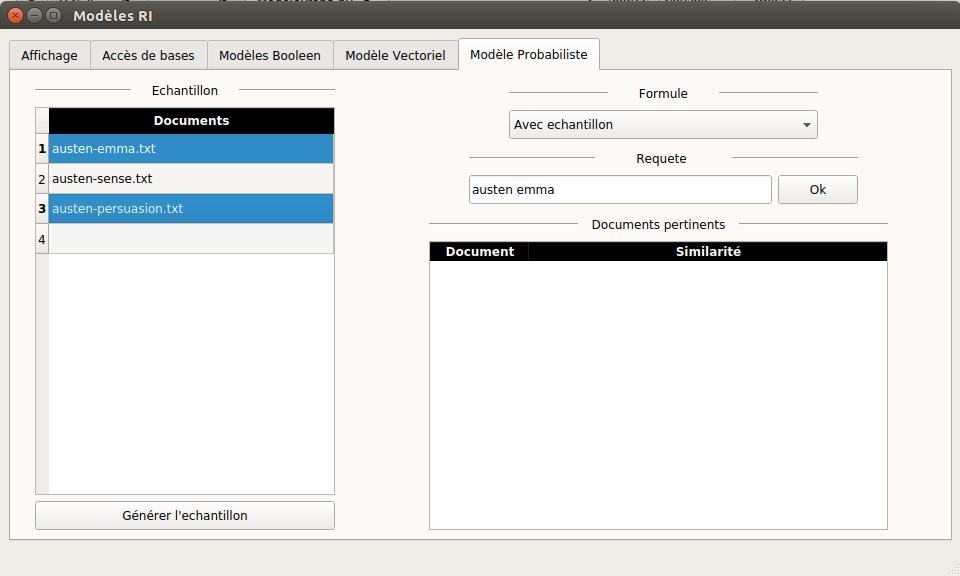
\includegraphics[scale=0.4]{images/modeleP.png}
		\caption{Affichage de l'échantillon et sélection de l'utilisateur.}
	\end{figure}
	
Maintenant que nous avons notre liste de documents pertinents, nous passons à l'application de la formule du modèle probabiliste, et cela en appuyant sur le bouton \textbf{"OK"} à coté de la requête.\\

Le résultat est donnée dans le tableau juste en dessous, tel que \textbf{les documents sont trié par ordre décroissant de similitude}.
	\begin{figure}[H]
		\centering
		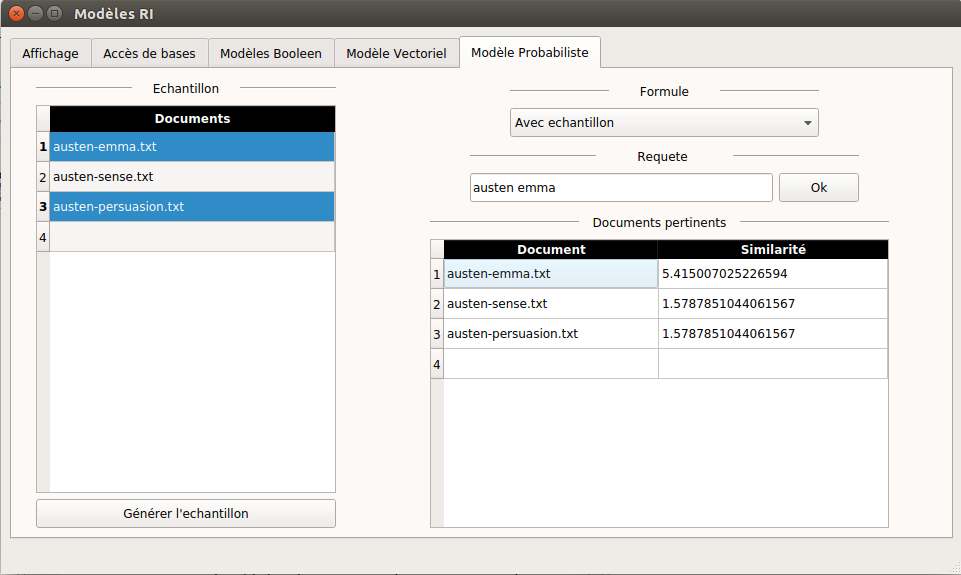
\includegraphics[scale=0.4]{images/modeleP2.png}
		\caption{Résultat du modèle probabiliste.}
	\end{figure}

\newpage 

\section{Bonus}

\subsection{Modèle Probabiliste sans échantillon}
Le principe étant assez proche du modèle probabiliste avec échantillon, à la différence de l'absence d'échantillon d'apprentissage comme son nom le précise.\\

De ce fait, la formule ne prend pas en compte les informations relatives à l'échantillon, tel qu'elle se présente comme suit:
\begin{center}
	Sim($d_{j},Q$)= $\sum_{i=1}^{n} P_{ij} * P_{iq} \log \dfrac{N-n_{i}+0.5}{n_{i}+0.5}$
\end{center}

\subsubsection*{Requête}
Identique à celle du modèle vectoriel et probabiliste avec échantillon.


\subsubsection*{Résultat}
Dans l'onglet dédié au modèle probabiliste de notre interface, nous avons une liste déroulante \textbf{ComboBox} nous permettant de sélectionner le \textbf{modèle Probabiliste sans échantillon}, puis procède normalement à la saisi de la requête et l'exécution de l'appariement.\\

Ainsi la liste des documents est retournée dans l'ordre décroissant de similitude, comme dans l'exécution suivante:

	\begin{figure}[H]
		\centering
		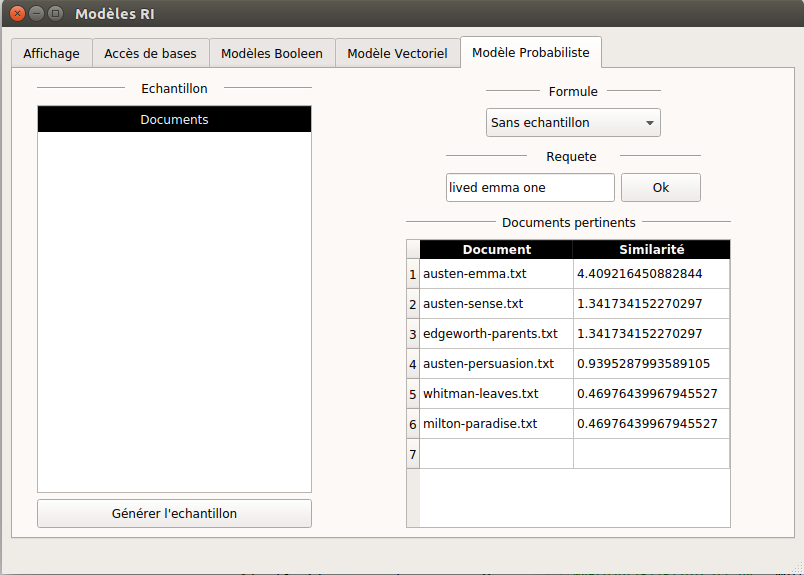
\includegraphics[scale=0.4]{images/modeleP3.png}
		\caption{Résultat du modèle probabiliste sans échantillon.}
	\end{figure}



\newpage

\subsection{Modèle Probabiliste BM25}
Il existe une variante du modèle probabiliste tout aussi utilisé \textbf{BM25}, aussi appelée l'estimation de \textbf{S.Walker}  \textbf{S.Roberston} qui à la différences des autres modèle prend en compte la longueur des documents ainsi que 2 constantes, la formule est donnée comme suit:
\begin{center}
	Sim($d_{j},Q$)= $\sum_{i=1}^{n} (\dfrac{(K+1)*freq_ij}{freq_ij + K*(1-B)+B*\frac{dl}{AVG dl}}) * \log \dfrac{N-n_{i}+0.5}{n_{i}+0.5}$
\end{center}

Avec:\\
$K: $Constante par defaut = 1.2.\\
$B: $Constante par défaut = 0.75.\\
$freq_ij :$fréquence du terme i dans le document j.\\
$dl: $ Longueur du document j.\\
$AVG dl: $ Longueur moyenne des documents de la collection.

\subsubsection*{Requête}
Identique à celle du modèle vectoriel et probabiliste avec et sans échantillon.



\subsubsection*{Résultat}
Toujours dans l'onglet du modèle probabiliste nous pouvons choisir l'option \textbf{BM25} de la liste défilante, insérer une requête et lancer l'évaluation de similitude afin d'obtenir les documents pertinents dans l'ordre décroissant de leur similitude.

	\begin{figure}[H]
		\centering
		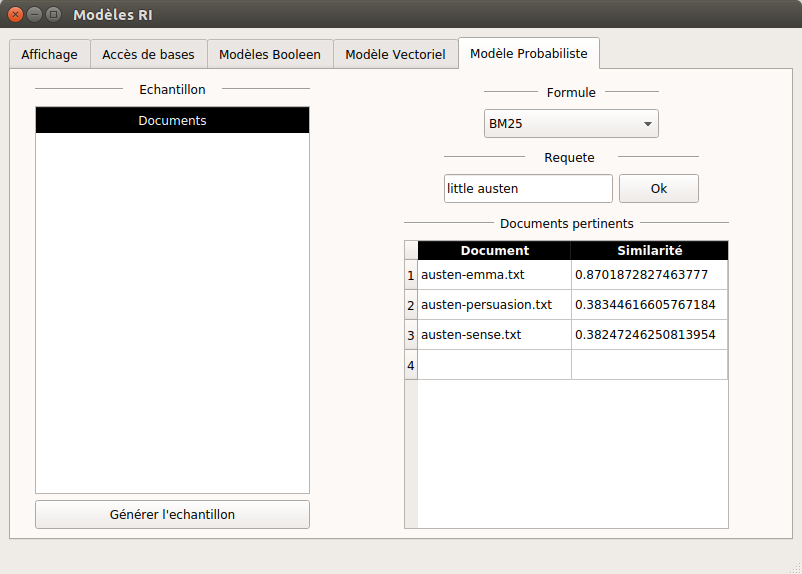
\includegraphics[scale=0.4]{images/modeleP4.png}
		\caption{Résultat du modèle BM25.}
	\end{figure}
\newpage

\section{Comparaison des trois modèles}
Après avoir étudié, implémenté et testé les 3 principaux modèles qui sont : \textbf{modèle booléen}, \textbf{modèle vectoriel} et \textbf{modèle probabiliste avec échantillon}, nous avons pu constater les avantages et inconvenants de chacun, citons:
\begin{itemize}
	\item[$\bullet$] le modèle est très rigide tel qu'il suffit qu'un seul terme de la requête de corresponde pas au contenu d'un document pour que ce dernier soit jugé non pertinent.
	
	Serte il ce peut que certain problème nécessite de genre de modèle, mais cela reste des cas particulier, en générale il est préférable d'avoir des documents ordonné par degrés de pertinence, ainsi il suffira de définir un seuil minimal pour éliminer les documents trop peu pertinent.
	
	\item[$\bullet$] le modèle vectoriel est bien plus souple que le précédent, il prend en compte le degrés de similitude et ceci peut être fait via une des 4 fonctions de calcule de similitude qu'il propose, soient : \textbf{Produit Interne}, \textbf{coefficient de Dice}, \textbf{Cosinus} et \textbf{Jaccard}.
	
	\item[$\bullet$] le modèle Probabiliste apporte une nouvelle notion \textbf{"d'échantillon"} tel que l'utilisateur peu influencer les similitudes des documents en précisant une liste de document qu'il juge lui même pertinents, et ce après connaissance de la collection a traiter.
	
	Ainsi ce modèle est encore plus souple et adaptable selon les besoins de l'utilisateur ce qui lui profère les meilleurs résultats en général, mais ce n'ai pas toujours possible de donner cette liberté à l'utilisateur, ce n'ai pas toujours facile pour l'utilisateur de reconnaitre les documents pertinents sur une large collection de documents.
\end{itemize}


\newpage

\section*{Conclusion}
En conclusion, après avoir passé en revu les différents modèles en mettant l'accent sur les avantages et inconvénients de chacun, nous déduisant que tous les modèles peuvent être jugé les plus performant selon le problème à résoudre et les ressources disponibles, car il n'y a pas de super modèle classé comme permettant d'obtenir les meilleurs résultats, et les plus précis pour tous les problèmes données.\\

Néanmoins nous pensons que lorsque nous ne savons pas quel modèle est le plus approprié il est préférable de se diriger vers le modèle vectoriel et selon l'évolution et les résultats décider s'il faut changer de modèle ou pas.\\

Aussi la création et manipulation des fichier inverse des fréquences et des poids permet une utilisation simple et structuré de nos données, d'ailleurs celles-ci permette une nette réduction du temps d'exécution et de recherche dans la collection de document.

\newpage

\section*{Références bibliographiques}

[1] : http://www.iro.umontreal.ca/~nie/IFT6255/historique-RI.html


\end{document}